\documentclass[conference]{IEEEtran}
\usepackage[utf8]{inputenc}
\usepackage[T1]{fontenc}
\usepackage{amsmath,amssymb}
\usepackage{graphicx}
\usepackage{booktabs}
\usepackage{multirow}
\usepackage{cite}
\usepackage{url}
\usepackage{xcolor}
\graphicspath{{figures/}}

\newcommand{\R}{\mathbb{R}}
\newcommand{\todo}[1]{\textcolor{red}{[TODO: #1]}}

\begin{document}

\title{Network-Aware Traffic Speed Forecasting on METR-LA:\\
Tree-Based Machine Learning Baselines and the Value of Road-Graph Information}

% Replace with the team's names, affiliation and e-mails before submission.
\author{\IEEEauthorblockN{Team T005}
\IEEEauthorblockA{\todo{author names, department, institution, e-mail}}}

\maketitle

\begin{abstract}
Short-term traffic forecasting asks how fast vehicles will move on each road segment minutes to an hour from now. We study this problem on METR-LA, a public benchmark of 207 loop detectors on Los Angeles highways recorded every five minutes for 119 days. This Phase~1 report covers the machine-learning component: a rigorous data audit, leakage-free feature engineering, three naive baselines, and three tree-ensemble learners (boosted trees that treat every sensor independently, a multi-output random forest, and boosted trees that additionally receive upstream and downstream neighbour speeds). Models are compared on a strictly chronological split, at 5, 15, 30 and 60 minutes, with MAE, RMSE and MAPE, separately for peak and off-peak periods, and with day-block bootstrap intervals. On 24 held-out days, boosted trees lower the mean absolute error by 18\% (5 min) to 32\% (60 min) relative to persistence; adding upstream and downstream neighbour speeds lowers it by a further 3.6\% to 1.8\% (95\% intervals exclude zero), and the multi-output random forest is 4.5\% to 13\% worse than boosting on MAE but matches or slightly beats it on RMSE. The study also quantifies which engineered feature groups carry the skill, documents a hyper-parameter search that uses only chronological validation, and states plainly what the data cannot support. The graph neural network and the signal-control simulation are Phase~2.
\end{abstract}

\begin{IEEEkeywords}
traffic forecasting, METR-LA, gradient boosting, random forest, feature engineering, chronological validation, spatial dependence
\end{IEEEkeywords}

%--------------------------------------------------------------------------------------------------
\section{Introduction}
Accurate forecasts of traffic speed support route guidance, incident response and signal planning. The difficulty is that congestion is not local: a slowdown that starts at one detector reaches the detectors upstream of it within minutes, and a model that forecasts every road segment from that segment's own history cannot see it coming. Whether explicit knowledge of the road network improves forecasts, and by how much, is the question that organises this project.

The full project has two phases. Phase~2 will train a graph attention network and a diffusion-based model over the road graph and add a simulated signal-control experiment. \emph{This report is Phase~1 and concerns the machine-learning component only.} Its purpose is to build the strongest conventional baseline that can be defended, to show exactly how it was validated, and to measure how much of the benefit of network structure a tree model captures when it is merely \emph{given} neighbour information as features. That measurement fixes the bar the graph models of Phase~2 have to clear.

\textbf{Contributions.}
(i)~A documented audit of METR-LA, including evidence that a reading of exactly zero encodes a missing observation rather than standstill traffic.
(ii)~A leakage-controlled forecasting setup: day-aligned chronological split, scaling fitted on the training period only, cyclic time features, masked outages, and executable checks of the temporal ordering.
(iii)~Three families of baselines (naive, boosted trees, random forest) and a spatial variant of the boosted model, evaluated under identical rules.
(iv)~A feature-group ablation with a seed-noise estimate, and a hyper-parameter study based on rolling-origin validation.
(v)~An explicit list of what the evidence does and does not establish.

%--------------------------------------------------------------------------------------------------
\section{Related Work}
\textbf{Classical and statistical forecasting.} Short-term traffic forecasting has a long history, surveyed by Vlahogianni et~al.~\cite{vlahogianni2014}. Seasonal ARIMA models treat the series of one detector as a univariate process whose weekly difference is stationary~\cite{williams2003}; they are cheap and interpretable but, like any per-detector model, ignore the network. Our naive baselines (persistence, rolling mean, seasonal average) play the role of these simple references.

\textbf{Tree ensembles and engineered features.} Gradient boosting~\cite{friedman2001gbm} and its scalable implementation XGBoost~\cite{chen2016xgboost} fit trees sequentially to the remaining error, while random forests~\cite{breiman2001rf} average decorrelated trees grown on bootstrap samples. Both handle heterogeneous tabular features, missing values and nonlinear interactions without feature scaling~\cite{hastie2009esl}, which is why they are the standard strong baselines when features are engineered from lagged measurements.

\textbf{Deep learning on traffic data.} Lv et~al.~\cite{lv2015} used stacked autoencoders on flow data. Models that use the road graph explicitly followed: DCRNN~\cite{li2018dcrnn}, which introduced METR-LA as a benchmark, models traffic as a diffusion process on a directed graph inside a recurrent encoder--decoder; STGCN~\cite{yu2018stgcn} combines graph and temporal convolutions; Graph WaveNet~\cite{wu2019graphwavenet} learns an adaptive adjacency matrix. These build on graph convolution~\cite{kipf2017gcn} and graph attention~\cite{velickovic2018gat}, the latter restricting self-attention to a node's neighbours. These models are the subject of Phase~2.

\textbf{Evaluation methodology.} For time series, random $k$-fold cross-validation leaks future information into training; Cerqueira et~al.~\cite{cerqueira2020} compare estimation protocols and find that out-of-sample (chronological) methods are the most reliable for non-stationary series. Because forecast errors are strongly autocorrelated, uncertainty must be estimated by resampling blocks rather than points~\cite{kunsch1989}. We follow both principles. Percentage errors are unstable near zero~\cite{hyndman2006}, so MAPE is computed only where the true speed is at least one mile per hour and reported with its own sample size.

\textbf{Simulation.} Signal-control studies use simulators such as SUMO~\cite{lopez2018sumo} and CityFlow~\cite{zhang2019cityflow}. Simulation belongs to Phase~2 and is simulation only; nothing in this project controls real traffic.

\textbf{Gap addressed.} Published graph models are usually compared with a few weak or untuned baselines. Here the independent-sensor baseline is made as strong as the data allow, a second tree family and a spatial tree variant are added, and the effect of every design choice is measured, so that any later gain of a graph model can be attributed to what it learns rather than to a weak reference.

%--------------------------------------------------------------------------------------------------
\section{Data and Exploratory Analysis}
\subsection{METR-LA}
METR-LA contains average speeds (mph) from 207 loop detectors on Los Angeles County highways, sampled every five minutes from 1~March to 27~June 2012: $34{,}272$ time steps, $7{,}094{,}304$ readings~\cite{li2018dcrnn}. A road-network distance file defines a directed sensor graph; we rebuild the weighted adjacency with the thresholded Gaussian kernel of DCRNN, which yields $1{,}515$ directed edges plus $207$ self-loops. Only speed is recorded: the brief mentions flow and occupancy, but this dataset has neither, and none is invented.

\subsection{Data quality}
\textbf{Zero means missing.} $8.11\%$ of all readings ($575{,}302$ cells) equal exactly $0.0$, while the smallest positive reading is $0.33$ mph and only $552$ readings lie in $(0,3)$ mph. In $2{,}148$ time steps ($6.27\%$) \emph{all 207} sensors read exactly zero simultaneously, which cannot be genuine traffic. We therefore convert zeros to missing values and keep an observation mask; no model ever treats an outage as zero speed.

\textbf{Structure of the gaps.} Missingness is mostly long: $68\%$ of missing cells belong to gaps between one hour and one day and $22.5\%$ to gaps of a day or more; the longest single gap is 5.8 days. Per-sensor missingness ranges from $6.3\%$ to $20.1\%$ and no sensor exceeds $50\%$. Missing data are not stationary: the test period has $12.0\%$ missing cells against $7.2\%$ in training (a factor of $1.68$), and $9.6\%$ of test windows contain no observation at all in the input window for the sensor concerned (training: $5.5\%$).

\textbf{Distribution and periodicity.} Observed speeds have mean $58.5$ mph, median $63.2$ mph and are capped at $70$ mph (the 99th percentile is $69.75$ mph); the distribution is strongly left-skewed because congestion produces a heavy tail of low speeds. Sensors differ widely: the per-sensor mean ranges from $30.9$ to $67.7$ mph. Weekdays are slower than weekends ($57.2$ vs.\ $61.6$ mph network mean), and the six slowest weekday hours are 08--09 and 15--18. The mean weekday speed inside the commute windows 07:00--10:00 and 15:00--19:00 is $50.4$ mph against $60.0$ mph outside them. These windows, which define \emph{peak} throughout, were fixed from this profile before any model was trained.

\begin{figure}[t]
\centering
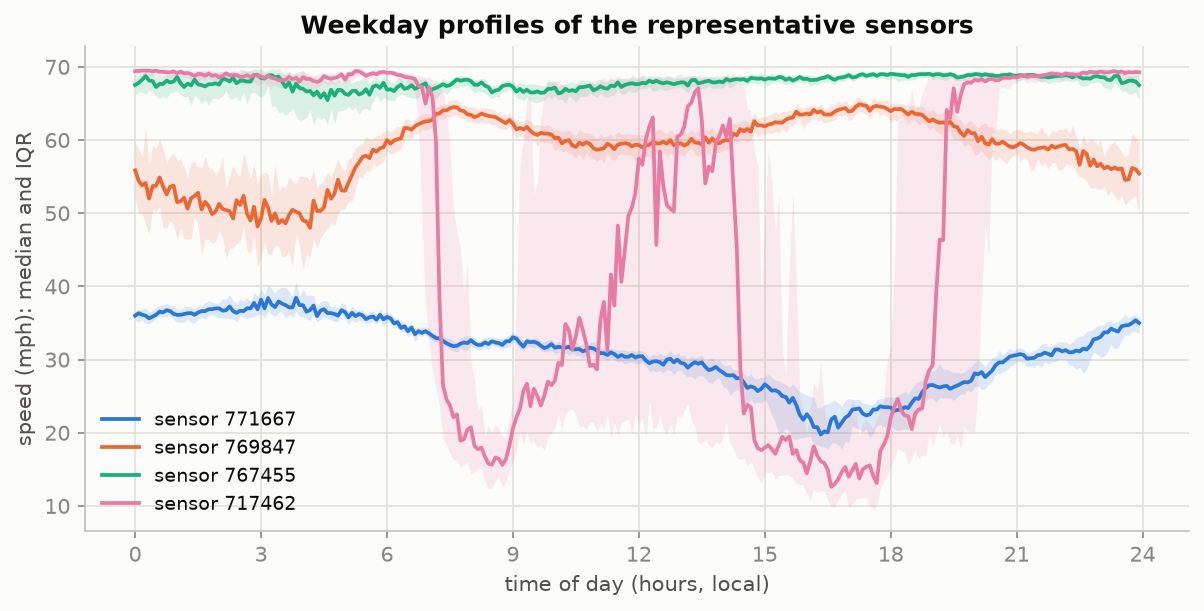
\includegraphics[width=\columnwidth]{eda_weekday_profile.png}
\caption{Weekday median speed and interquartile range of four representative sensors (slowest, median, fastest and most variable by training statistics). Sensor behaviour differs strongly; the most variable sensor shows the morning and afternoon congestion that defines the peak windows.}
\label{fig:profile}
\end{figure}

\begin{figure*}[t]
\centering
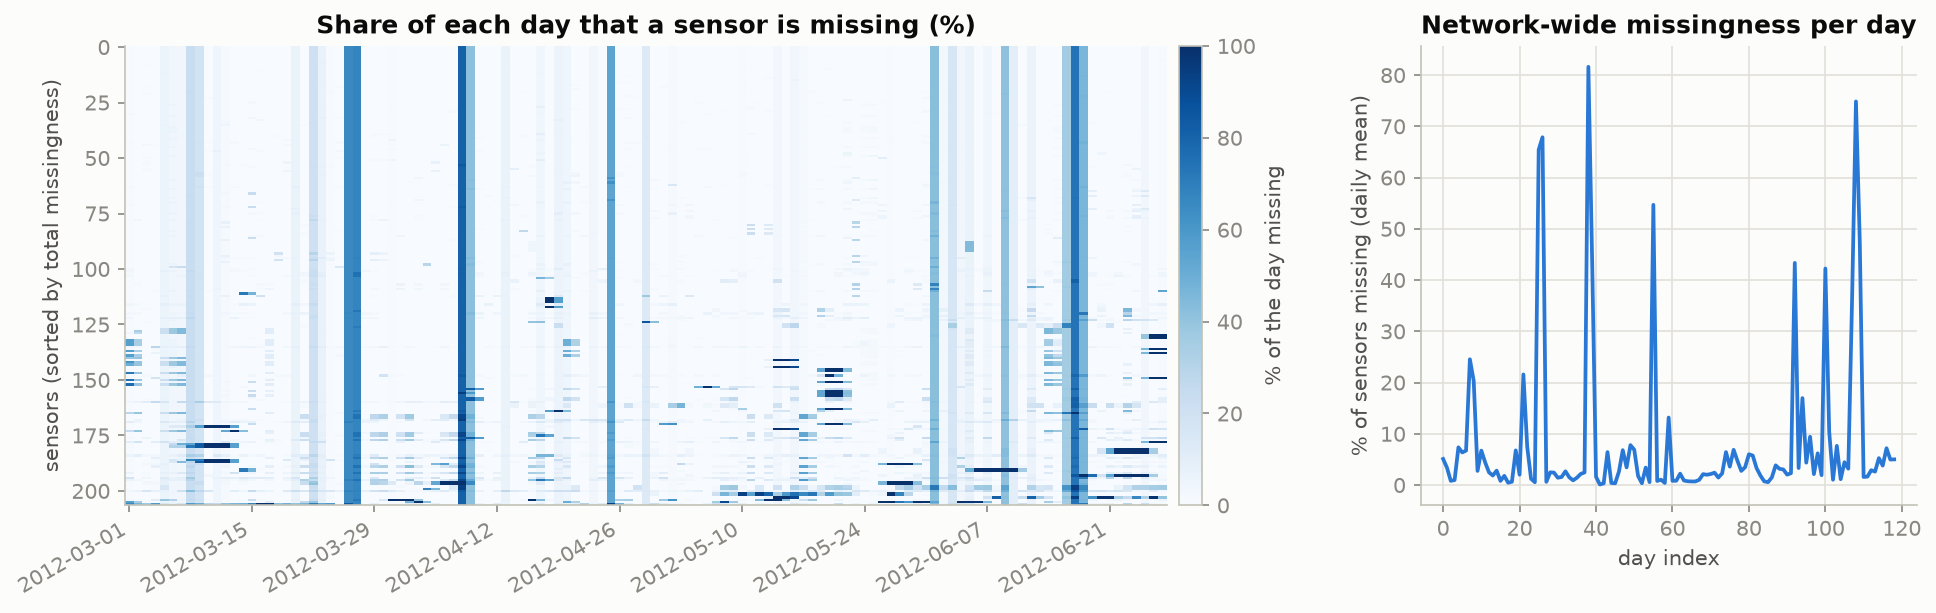
\includegraphics[width=\textwidth]{eda_missingness.png}
\caption{Missing readings. Left: share of each day that each sensor is missing (sensors sorted by total missingness). Right: network-wide missingness per day. Vertical bands are network-wide outages; horizontal bars are single-sensor failures. Missing data are bursty, not random.}
\label{fig:missing}
\end{figure*}

\subsection{Limitations of the dataset}
One city, 119 days in 2012, speed only, 207 of roughly four thousand detectors, a speed cap at 70 mph, naive (zone-less) timestamps for which Pacific local time is assumed, and no incident, weather or holiday labels. The copy of the data used here was obtained from a third-party mirror because the original is distributed through file-sharing links; its structure, 5-minute grid and sensor order were validated against the DCRNN files, but the file was not compared byte for byte. Conclusions are therefore about this network and period.

%--------------------------------------------------------------------------------------------------
\section{Problem Formulation and Theoretical Background}
\subsection{Formulation}
Let $v_{t,n}$ be the speed of sensor $n$ at step $t$ and $m_{t,n}\in\{0,1\}$ its observation mask. From the last $L=12$ steps (60 minutes) we forecast $v_{t+h,n}$ for $h\in\{1,3,6,12\}$ steps, i.e.\ 5, 15, 30 and 60 minutes ahead. A forecast origin $t$ is valid for a split only if all its targets $t+1,\dots,t+12$ lie inside that split; its inputs may reach back into an earlier split, which is legitimate because past data are available at forecast time.

\subsection{Residual formulation and the persistence anchor}
Let $a_{t,n}$ be the latest observed speed of sensor $n$ in the input window (the training mean of the sensor if the whole window is missing). Persistence forecasts $\hat v_{t+h,n}=a_{t,n}$. All learned models predict the residual
\begin{equation}
r_{t+h,n}=v_{t+h,n}-a_{t,n},\qquad \hat v_{t+h,n}=a_{t,n}+\hat r_{t+h,n},
\end{equation}
so every model is judged on what it adds beyond persistence, and the trees only need to learn the change of speed rather than the level.

\subsection{Gradient boosting (XGBoost)}
Boosting builds an additive model $F_M(x)=\sum_{m=1}^{M}\eta f_m(x)$ of regression trees with shrinkage $\eta$, each tree fitted to reduce the loss left by its predecessors~\cite{friedman2001gbm}. XGBoost minimises a regularised objective $\sum_i \ell(y_i,\hat y_i)+\sum_m\Omega(f_m)$ with $\Omega(f)=\gamma T+\tfrac12\lambda\lVert w\rVert^2$ for a tree with $T$ leaves and leaf weights $w$. A second-order expansion gives, for a leaf whose samples have gradient sum $G$ and Hessian sum $H$, the optimal weight $w^{*}=-G/(H+\lambda)$, and the gain of a split into left and right parts
\begin{equation}
\tfrac12\Big[\tfrac{G_L^2}{H_L+\lambda}+\tfrac{G_R^2}{H_R+\lambda}-\tfrac{(G_L+G_R)^2}{H_L+H_R+\lambda}\Big]-\gamma .
\end{equation}
The split with the largest gain is taken, and $\gamma$, $\lambda$, the maximum depth and the minimum child weight limit overfitting~\cite{chen2016xgboost}. We train with the absolute-error objective, whose minimiser is the conditional \emph{median}, so the optimised loss is the evaluation metric (MAE). Because that loss has no useful curvature, XGBoost fits the trees to its (sub)gradient and updates the leaf values from the residuals in the leaf. Missing feature values are routed along a learned default direction at every split, so lagged values from an outage stay missing instead of being imputed.

One boosted model is fitted \emph{per horizon} (the direct multi-step strategy): there is no error accumulation as in recursive forecasting, at the price of four fits. A single global model is shared by all sensors, with a categorical sensor identifier, coordinates and the sensor's training mean as features, rather than $207\times4$ small per-segment models, each of which would see about $10^{5}$ correlated rows.

\subsection{Random forest}
A random forest averages $B$ trees grown on bootstrap samples, with a random subset of features considered at each split~\cite{breiman2001rf}. If the trees have variance $\sigma^2$ and pairwise correlation $\rho$, the variance of their average is
\begin{equation}
\rho\sigma^2+\frac{1-\rho}{B}\sigma^2 ,
\end{equation}
so averaging removes the second term and feature subsampling reduces $\rho$~\cite{hastie2009esl}; unlike boosting, bagging does not reduce bias. In scikit-learn~\cite{pedregosa2011sklearn} the forest supports several outputs natively: a split is chosen to minimise the \emph{summed} squared error of all outputs, so the four horizons share one tree structure. Two consequences matter for interpretation. First, the squared-error criterion estimates a conditional \emph{mean}, whereas the metric of interest is MAE, so the forest optimises a related but different quantity than XGBoost. Second, a forest cannot learn from a partly missing target vector, so only rows whose targets are observed at all four horizons are used for fitting; scoring still uses every observed target. Missing feature values are handled natively. Impurity-based importances are biased towards features with many distinct values~\cite{strobl2007}; we therefore also report permutation importance on the validation period.

\subsection{Why the chronological protocol matters}
Random shuffling would place a window ending at 08:00 in training and its neighbour ending at 08:05 in validation; the two share eleven of twelve inputs and most of their targets, which would reward memorisation. All splits are therefore made on whole days in time order: $83$ training days (1~Mar--22~May), $12$ validation days (23~May--3~Jun) and $24$ test days (4--27~Jun), i.e.\ $69.7\%/10.1\%/20.2\%$. Training windows never contain a target from validation or test. The test period is touched only for the final scoring, once.

For model selection inside the training period we use \emph{rolling-origin} validation: the origins are cut into consecutive blocks, fold $i$ trains on blocks $1..i{-}1$ and validates on block $i$, and training origins whose farthest target $t+12$ reaches the first validation origin are removed (a gap), so no training target overlaps a validation target.

\subsection{Metrics and uncertainty}
With $\mathcal V$ the set of valid (observed target, finite forecast, common to all models) points,
\begin{align}
\mathrm{MAE}&=\tfrac{1}{|\mathcal V|}\sum_{\mathcal V}|\hat v-v|,&
\mathrm{RMSE}&=\sqrt{\tfrac{1}{|\mathcal V|}\sum_{\mathcal V}(\hat v-v)^2},\\
\mathrm{MAPE}&=\tfrac{100}{|\mathcal V'|}\sum_{\mathcal V'}\tfrac{|\hat v-v|}{v},
\end{align}
with $\mathcal V'=\{v\ge 1\ \text{mph}\}\subseteq\mathcal V$. Forecasts of every model are clipped to $[0,70]$ mph before scoring. The relative improvement of a candidate over a reference is $100\,(e_{\rm ref}-e_{\rm cand})/e_{\rm ref}$, positive when the candidate is better. Its 95\% interval comes from a day-block bootstrap: whole test days are resampled with replacement ($2000$ replicates), because errors within one day are strongly correlated and resampling individual points would give overconfident intervals~\cite{kunsch1989}.

%--------------------------------------------------------------------------------------------------
\section{Feature Engineering}
Every feature uses readings at or before the forecast origin; calendar information about the \emph{target} time is allowed because it is known in advance. One row is one (origin, sensor) pair. Table~\ref{tab:features} lists the groups.

\begin{table}[t]
\centering
\caption{Engineered features (one row per origin and sensor).}
\label{tab:features}
\small
\begin{tabular}{@{}p{2.6cm}p{5.2cm}@{}}
\toprule
Group & Content \\
\midrule
Lags & speeds at lags 0--11 (NaN where missing) \\
Rolling statistics & mean over 3, 6, 12 steps; std over 6, 12 steps; number observed; short trend (mean of last 3 minus the 3 before) \\
Anchor & last observed speed in the window; its age in steps \\
Calendar & sin/cos of time of day and of day of week of the target; weekend flag \\
Sensor identity & training-mean speed, latitude, longitude, categorical id \\
Road-graph neighbours & upstream / downstream weighted mean speed now and 15 min earlier, slowest neighbour, number observed \\
\bottomrule
\end{tabular}
\end{table}

Cyclic encoding makes 23:55 and 00:00 neighbours; the speed scaler, the per-sensor training mean and every statistic are fitted on training timestamps only, and a test of the pipeline corrupts validation and test data and checks that nothing changes. A seasonal-average feature was deliberately \emph{not} used: a mean fitted on the training rows contains the training target itself, which creates an in-sample advantage the model does not have at test time. Neighbour features are computed from the directed graph: upstream neighbours are sensors $j$ with an edge $j\to i$, downstream neighbours the reverse, with edge weights as weights in the mean; only readings at or before the origin are used and missing neighbours are skipped.

%--------------------------------------------------------------------------------------------------
\section{Experimental Setup}
\textbf{Models.} (1)~Persistence; (2)~rolling mean of the last 60 minutes; (3)~seasonal average by weekday and time slot fitted on training data; (4)~XGBoost, independent sensors; (5)~multi-output random forest; (6)~XGBoost with road-graph neighbour features; and, when the search finds a clearly better configuration, (7)~tuned XGBoost.

\textbf{Fair comparison.} All models use the same origins, horizons, 60-minute history window, targets, mask and scoring code. Validation (never test) is used for early stopping and for every choice. The random forest has 150 trees; its minimum leaf size (5), share of features per split (0.7) and share of rows per tree (0.3) were chosen from a six-setting grid on validation data only. The boosted models use $\eta=0.08$, depth~8, minimum child weight~20, row and column subsampling $0.8$, $\lambda=5$, up to $1500$ rounds with early stopping after $40$ rounds without validation improvement.

\textbf{Hardware and reproducibility.} All code is in \texttt{src/} with tests; seeds are fixed (42); data checksums are in the repository.

%--------------------------------------------------------------------------------------------------
\section{Results}
\begin{table*}[t]
\centering
\caption{Test-period error by forecast horizon (24 held-out days, 207 sensors). MAE and RMSE in mph, MAPE in \%; lower is better, best per column in bold. All models are scored on the same valid points.}
\label{tab:main}
\small
\begin{tabular}{@{}lrrrrrrrrrrrr@{}}
\toprule
 & \multicolumn{4}{c}{MAE (mph)} & \multicolumn{4}{c}{RMSE (mph)} & \multicolumn{4}{c}{MAPE (\%)} \\
\cmidrule(lr){2-5}\cmidrule(lr){6-9}\cmidrule(lr){10-13}
Model & 5 min & 15 min & 30 min & 60 min & 5 min & 15 min & 30 min & 60 min & 5 min & 15 min & 30 min & 60 min \\
\midrule
Persistence & 2.82 & 3.49 & 4.19 & 5.35 & 4.61 & 6.38 & 7.98 & 10.25 & 6.47 & 8.57 & 10.79 & 14.42 \\
Rolling mean (60 min) & 3.44 & 3.92 & 4.55 & 5.66 & 6.52 & 7.58 & 8.85 & 10.80 & 9.11 & 10.59 & 12.55 & 15.96 \\
Seasonal average & 4.18 & 4.18 & 4.18 & 4.18 & 7.83 & 7.83 & 7.83 & 7.83 & 12.97 & 12.97 & 12.97 & 12.97 \\
Random forest (multi-output) & 2.41 & 3.02 & 3.55 & 4.14 & 4.05 & 5.47 & 6.45 & 7.40 & 5.89 & 8.11 & 10.07 & 12.32 \\
XGBoost & 2.30 & 2.83 & 3.25 & 3.66 & 4.04 & 5.54 & 6.57 & 7.44 & 5.63 & 7.59 & 9.47 & 11.40 \\
XGBoost (tuned) & 2.30 & 2.82 & 3.23 & 3.61 & 4.04 & 5.52 & 6.55 & 7.37 & 5.62 & 7.56 & 9.40 & 11.14 \\
XGBoost + neighbours & \textbf{2.22} & \textbf{2.74} & \textbf{3.16} & \textbf{3.60} & \textbf{3.81} & \textbf{5.24} & \textbf{6.28} & \textbf{7.21} & \textbf{5.29} & \textbf{7.26} & \textbf{9.06} & \textbf{11.01} \\
\bottomrule
\end{tabular}
\end{table*}


\textbf{Overall ranking.} Table~\ref{tab:main} and Fig.~\ref{fig:horizon} give the test errors. Every learned model beats persistence at every horizon on MAE, and the error of every model grows with the horizon. Boosted trees reduce the MAE of persistence from 2.82, 3.49, 4.19 and 5.35 mph to 2.30, 2.83, 3.25 and 3.66 mph at 5, 15, 30 and 60 minutes. The seasonal average, which ignores the current state, has a constant 4.18 mph MAE: worse than persistence at short horizons, level with it at 30 minutes and better at 60 minutes, but worse than boosting everywhere. The 60-minute rolling mean is worse than persistence at every horizon: smoothing adds lag to a series that changes quickly. XGBoost with neighbour features is the best model on all three metrics at all four horizons.

\begin{figure*}[t]
\centering
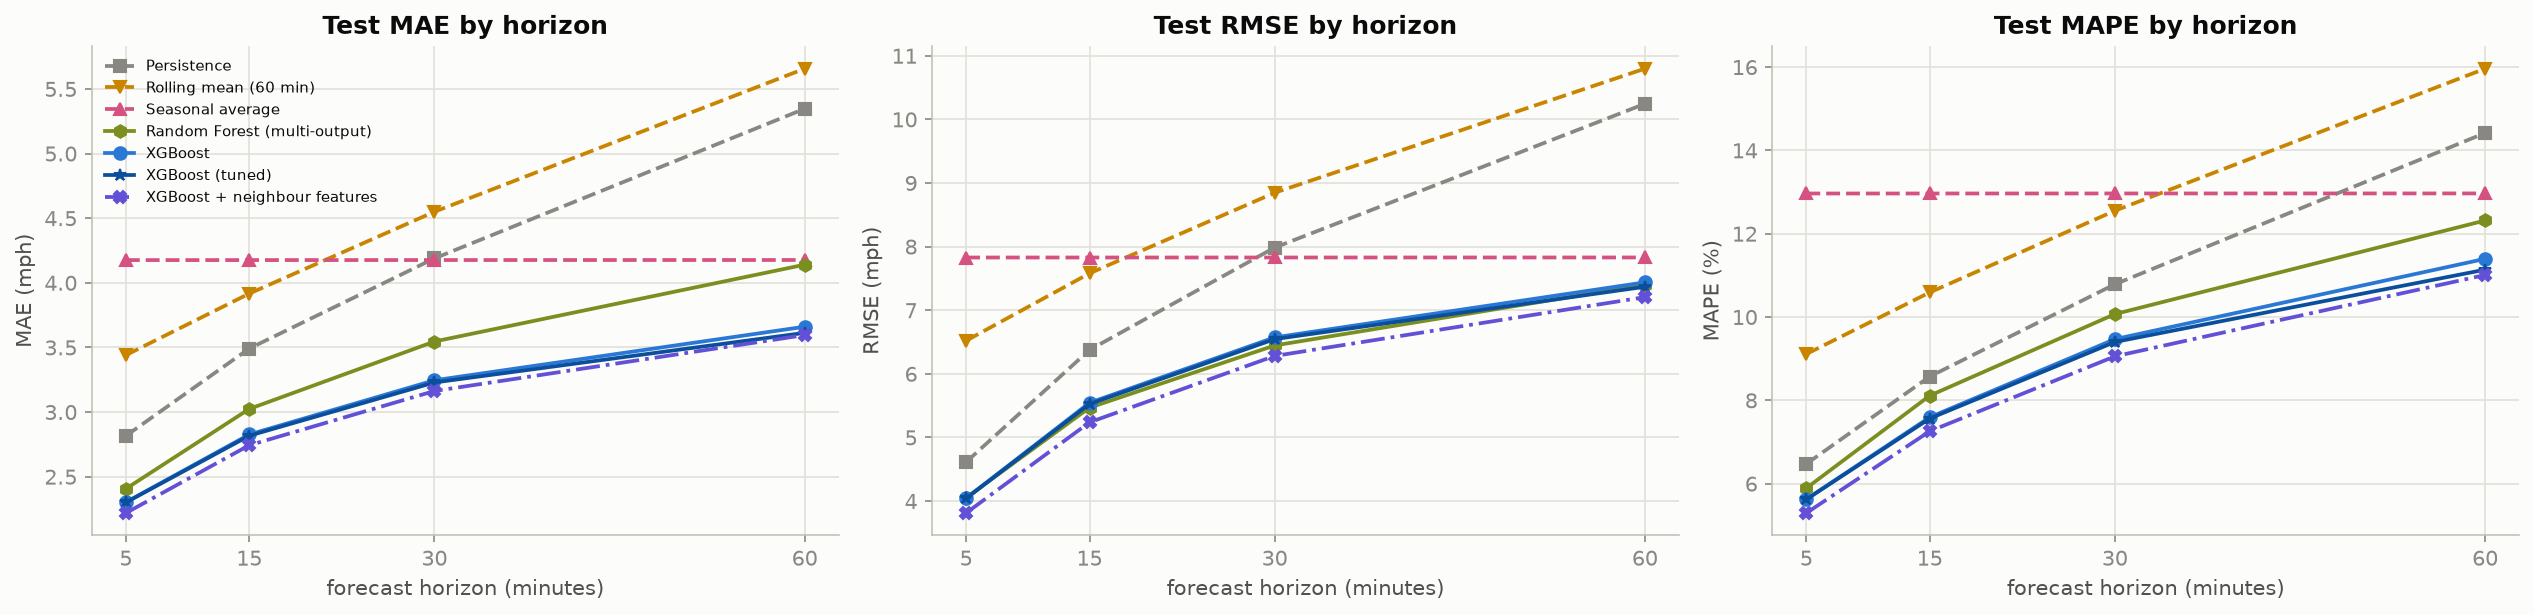
\includegraphics[width=\textwidth]{results_by_horizon.png}
\caption{Test MAE, RMSE and MAPE by forecast horizon for all Phase~1 models.}
\label{fig:horizon}
\end{figure*}

\begin{table*}[t]
\centering
\caption{MAE improvement (\%) of the first model over the second, with 95\% day-block bootstrap interval. Positive means the first model is better; an interval that excludes zero is a consistent difference over the 24 test days.}
\label{tab:improve}
\small
\begin{tabular}{@{}lrrrr@{}}
\toprule
Comparison & 5 min & 15 min & 30 min & 60 min \\
\midrule
XGBoost vs.\ persistence & 18.2 [17.7, 18.8] & 19.0 [18.4, 19.7] & 22.5 [21.4, 23.5] & 31.5 [29.3, 33.3] \\
Random forest vs.\ XGBoost & -4.5 [-4.9, -4.2] & -7.0 [-7.6, -6.6] & -9.2 [-10.1, -8.5] & -13.1 [-14.5, -11.8] \\
XGB + neighbours vs.\ XGBoost & 3.6 [3.3, 4.0] & 2.9 [2.7, 3.2] & 2.6 [2.2, 2.9] & 1.8 [1.4, 2.2] \\
XGB + neighbours vs.\ random forest & 7.8 [7.5, 8.0] & 9.3 [9.0, 9.7] & 10.8 [10.3, 11.4] & 13.2 [12.3, 14.1] \\
Tuned vs.\ default XGBoost & 0.1 [0.1, 0.1] & 0.3 [0.3, 0.4] & 0.5 [0.4, 0.6] & 1.3 [1.0, 1.5] \\
\bottomrule
\end{tabular}
\end{table*}


\textbf{Uncertainty.} Table~\ref{tab:improve} reports MAE improvements with day-block bootstrap intervals. Boosting versus persistence ($+18\%$ to $+32\%$) and neighbour features versus plain boosting ($+3.6\%$ to $+1.8\%$) are consistent over the 24 test days, as is the deficit of the random forest. The tuned configuration improves on the default by $0.1\%$ to $1.3\%$; the intervals exclude zero but the effect is small in absolute terms (at most 0.04 mph).

\textbf{Boosting versus bagging.} The random forest has a 4.5\% to 13.1\% higher MAE than XGBoost, yet an equal or slightly lower RMSE from 15 minutes on (15~min: 5.47 vs.\ 5.54~mph; 30~min: 6.45 vs.\ 6.57~mph; 60~min: 7.40 vs.\ 7.44~mph). The pattern fits the training objectives, although we did not test the explanation by swapping them: squared-error splits target the conditional mean, which minimises RMSE, whereas the absolute-error objective targets the conditional median, which minimises MAE and also helped MAPE. Which of the two is better therefore depends on the metric, and a single-number comparison would hide this. A permutation-importance analysis of the forest (Fig.~\ref{fig:rfimp}) ranks the last observed speed first (31\% of the total), followed by time of day, the sensor's mean speed and the current speed; the impurity ranking broadly agrees but assigns more weight to features with many distinct values, such as the sine of time of day (6.8\% vs.\ 4.3\%).

\begin{figure}[t]
\centering
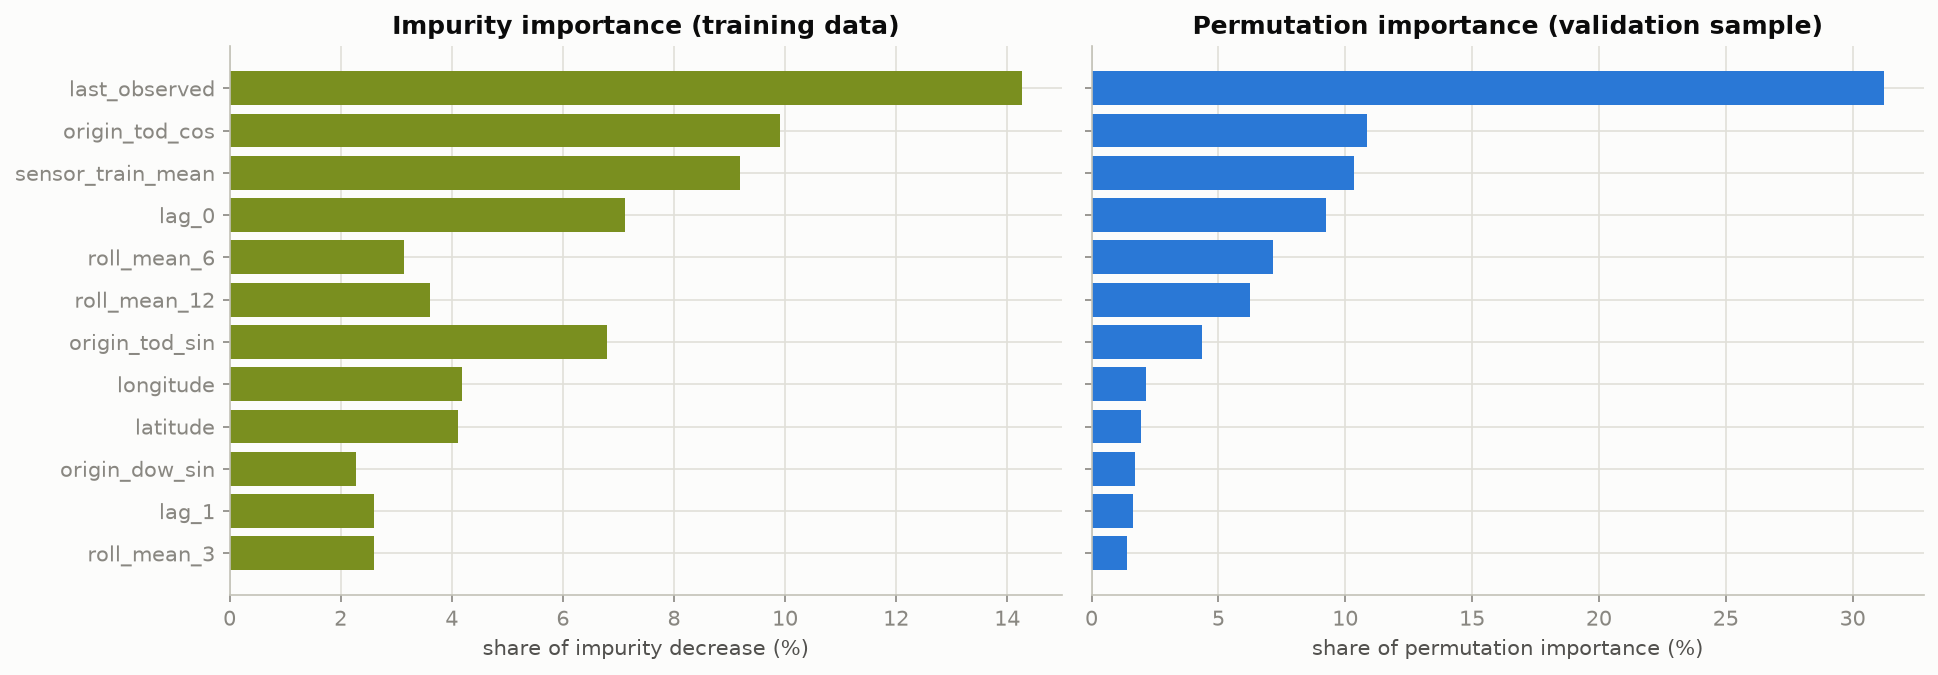
\includegraphics[width=\columnwidth]{rf_importance.png}
\caption{Random-forest feature importance: impurity decrease on training data (left) and permutation importance on a validation sample (right).}
\label{fig:rfimp}
\end{figure}

\begin{table}[t]
\centering
\caption{Test MAE (mph) in weekday peak hours (07--10, 15--19, by forecast target time) and all other hours.}
\label{tab:peak}
\small
\begin{tabular}{@{}llrrrr@{}}
\toprule
Period & Model & 5 min & 15 min & 30 min & 60 min \\
\midrule
\multirow{5}{*}{peak} & Persistence & 3.31 & 4.59 & 5.82 & 7.74 \\
 & XGBoost & 2.92 & 3.98 & 4.83 & 5.67 \\
 & Random forest (multi-output) & 3.05 & 4.25 & 5.25 & 6.42 \\
 & XGBoost + neighbours & 2.74 & 3.79 & 4.63 & 5.50 \\
 & XGBoost (tuned) & 2.92 & 3.96 & 4.79 & 5.55 \\
\midrule
\multirow{5}{*}{off-peak} & Persistence & 2.66 & 3.16 & 3.69 & 4.62 \\
 & XGBoost & 2.11 & 2.48 & 2.76 & 3.05 \\
 & Random forest (multi-output) & 2.21 & 2.65 & 3.03 & 3.45 \\
 & XGBoost + neighbours & 2.06 & 2.42 & 2.72 & 3.02 \\
 & XGBoost (tuned) & 2.11 & 2.47 & 2.75 & 3.02 \\
\bottomrule
\end{tabular}
\end{table}


\textbf{Peak versus off-peak.} All models make larger errors in the weekday peaks (Table~\ref{tab:peak}, Fig.~\ref{fig:peak}): for XGBoost the 5-minute MAE is 2.92 mph in peak hours against 2.11 mph otherwise, and the 60-minute MAE is 5.67 against 3.05 mph. Peak hours make up 23.3\% of the scored points. Relative to persistence, XGBoost gains about 12\% in peak hours and 21\% off-peak at 5 minutes, and 27\% against 34\% at 60 minutes, so the hardest periods are also those where a sensor-local model helps least. Neighbour information pays off most when it matters most: at 5 minutes it lowers the XGBoost MAE by 2.92$\to$2.74 mph in the peaks but only 2.11$\to$2.06 mph off-peak.

\begin{figure*}[t]
\centering
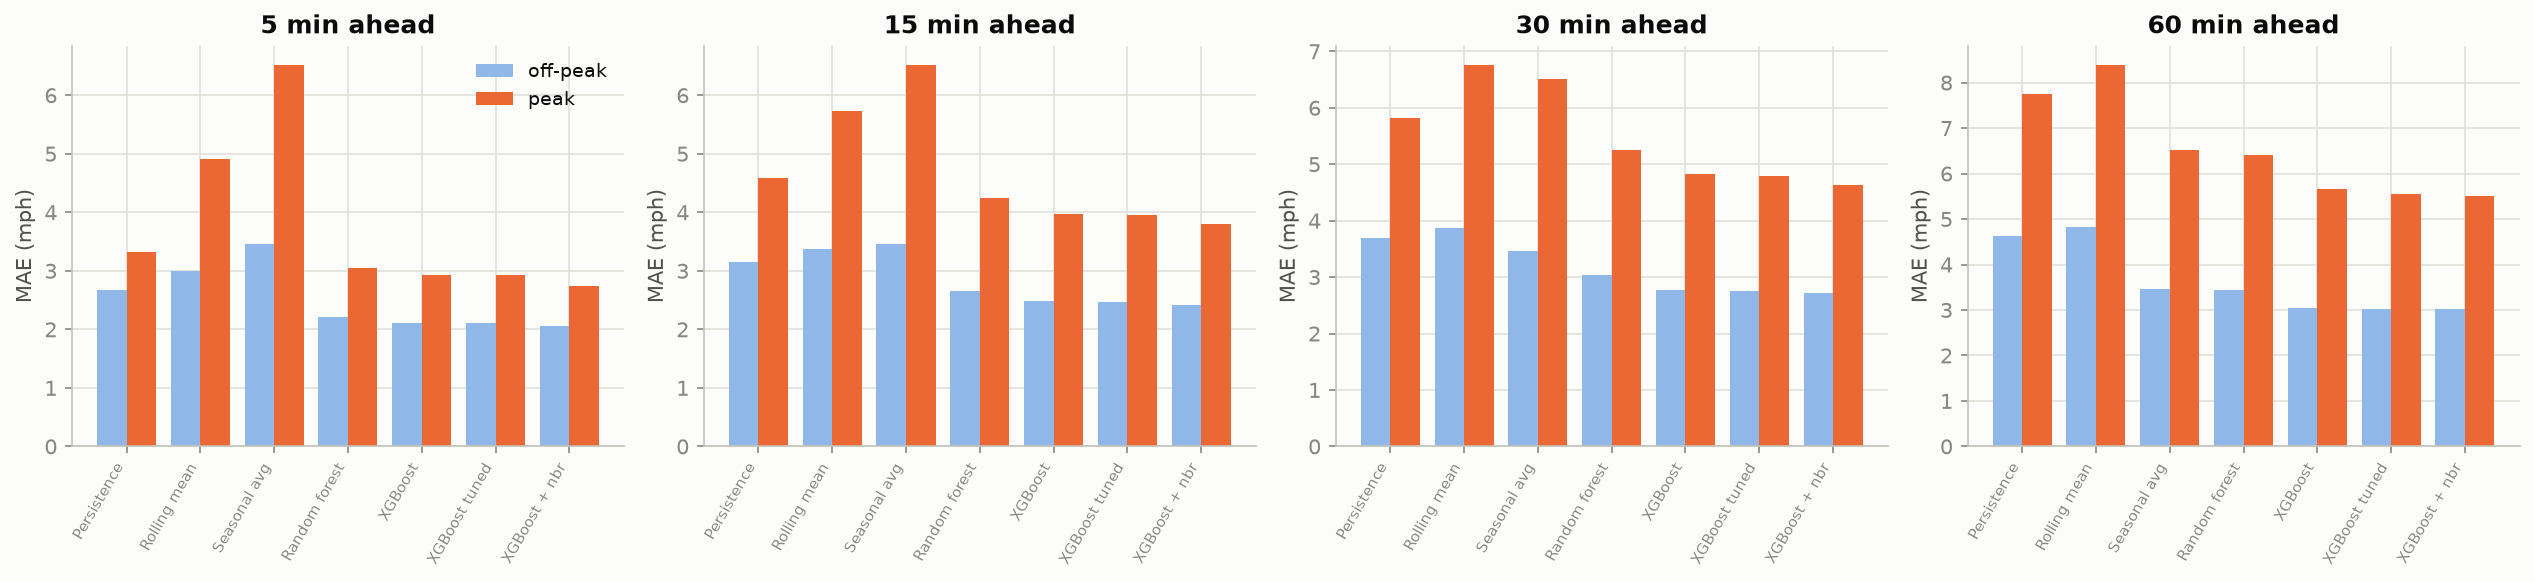
\includegraphics[width=\textwidth]{peak_vs_offpeak.png}
\caption{Test MAE in peak and off-peak hours for each model and horizon.}
\label{fig:peak}
\end{figure*}

\begin{table*}[t]
\centering
\caption{Cumulative feature-group ablation (validation MAE in mph; gain relative to the previous stage in \%). Persistence on the same rows is the reference.}
\label{tab:ablation}
\small
\begin{tabular}{@{}lrrrr@{}}
\toprule
 & \multicolumn{2}{c}{15 min} & \multicolumn{2}{c}{60 min} \\
\cmidrule(lr){2-3}\cmidrule(lr){4-5}
Stage & MAE & gain & MAE & gain \\
\midrule
1 lags + last value & 2.819 & 12.7 & 4.382 & 9.3 \\
2 + rolling stats, trend & 2.818 & 0.0 & 4.381 & 0.0 \\
3 + calendar (target time) & 2.746 & 2.5 & 3.984 & 9.1 \\
4 + sensor identity & 2.676 & 2.6 & 3.575 & 10.3 \\
5 + road-graph neighbours & 2.604 & 2.7 & 3.514 & 1.7 \\
\bottomrule
\end{tabular}
\end{table*}


\textbf{Which features carry the skill.} Table~\ref{tab:ablation} and Fig.~\ref{fig:ablation} add feature groups cumulatively. The 12 lags and the last observed value already reduce the validation MAE by 12.7\% (15 min) and 9.3\% (60 min) relative to persistence. The rolling statistics and trend add essentially nothing on top (0.05\% and 0.02\%), which is inside the seed-to-seed noise of the full model (standard deviation 0.001 and 0.004 mph over three seeds). Calendar features and sensor identity matter a great deal at long horizons: 9.1\% and 10.3\% at 60 minutes, against 2.5\% and 2.6\% at 15 minutes. The neighbour features add 2.7\% at 15 minutes and 1.7\% at 60 minutes. At one hour ahead, knowing \emph{when} and \emph{where} a forecast is made is worth far more than knowing the speed at the neighbouring detectors. The stages are cumulative, so the gains depend on the order in which the groups are added.

\begin{figure}[t]
\centering
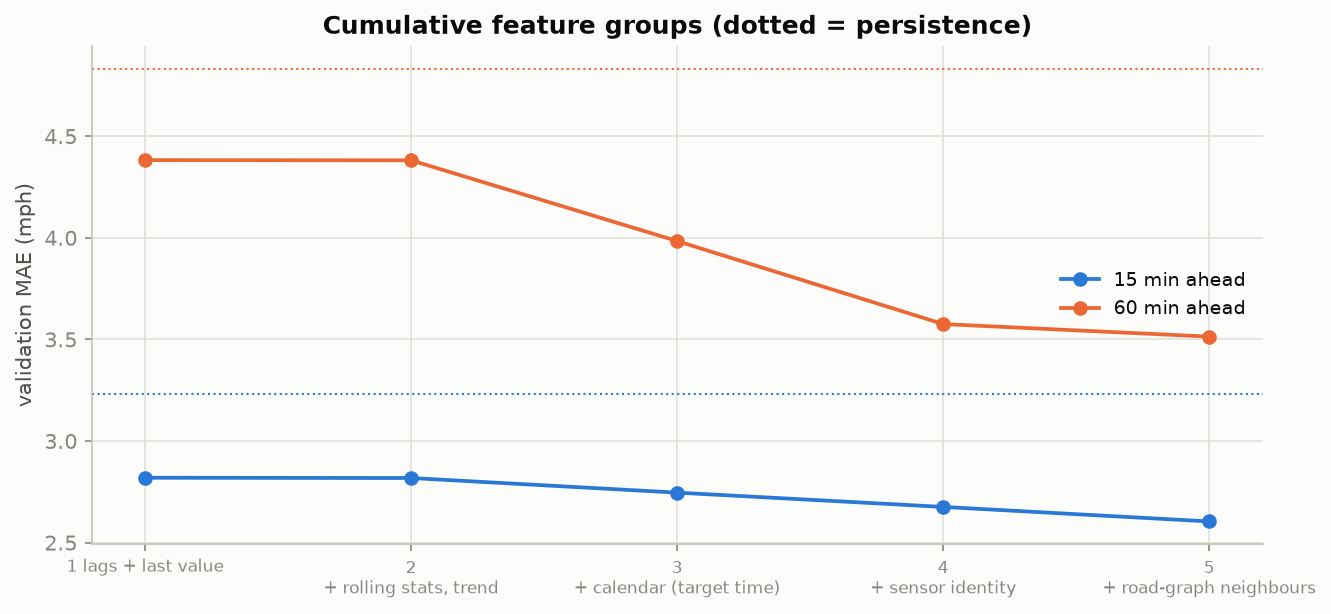
\includegraphics[width=\columnwidth]{feature_ablation.png}
\caption{Validation MAE as feature groups are added; dotted lines show persistence.}
\label{fig:ablation}
\end{figure}

\begin{table}[t]
\centering
\caption{Hyper-parameter study at 30 minutes. Rolling-origin cross-validation inside the training period for the default and the best random-search candidates (MAE of the residual, mph).}
\label{tab:tuning}
\small
\begin{tabular}{@{}lrrrrr@{}}
\toprule
Config. & depth & min.\ child & $\eta$ & CV MAE & vs.\ default (\%) \\
\midrule
cfg11 & 10 & 50 & 0.08 & 3.2350 & +0.54 \\
cfg05 & 10 & 50 & 0.08 & 3.2355 & +0.52 \\
cfg12 & 10 & 20 & 0.05 & 3.2405 & +0.37 \\
default & 8 & 20 & 0.08 & 3.2525 & +0.00 \\
\bottomrule
\end{tabular}
\end{table}


\textbf{Hyper-parameter study.} Twelve random candidates and the default were compared at 30 minutes on a thinned training set (validation MAE between 3.08 and 3.24 mph; the default scored 3.094). The three best candidates and the default were then cross-validated inside the training period with three rolling-origin folds (Table~\ref{tab:tuning}). The best challenger lowered the mean cross-validation MAE by 0.54\% and won all three folds, just above the pre-set adoption threshold of 0.5\%, and was refitted for all horizons. The lesson is not the winner but the flatness of the surface: the default configuration was within about 0.4\% of the best searched value, so tuning does not change any conclusion.

%--------------------------------------------------------------------------------------------------
\section{Discussion}
\textbf{Does network information help a conventional model?} Yes, modestly and consistently. Giving a tree model the speeds of the neighbouring detectors lowers the MAE by $3.6\%$ at 5 minutes and $1.8\%$ at 60 minutes, and the RMSE by $5.7\%$ and $3.1\%$, and the gain is concentrated in peak hours, when congestion propagates. This is the practical meaning of the gap stated in the introduction: part of what an independent-sensor model misses is available to it as soon as it is told what the upstream and downstream detectors read. It also means that a graph model must be compared with the spatially informed tree model, not only with the independent one; only a gain over \emph{that} reference shows that the graph model learns something beyond neighbour speeds.

\textbf{Why the independent model is already strong.} Most of the skill is recurrent: a sensor's own level, the time of day and the last observation explain the bulk of the improvement over persistence, especially at one hour. The dynamic information that the lags carry appears to be largely captured by the last value and a few recent lags, a plausible reason why rolling summaries add nothing.

\textbf{Metric choice matters.} The forest's MAE deficit alongside an RMSE tie, and the larger RMSE than MAE gains of neighbour features (consistent with neighbour information mattering most for large errors), show that reporting a single metric would change conclusions; we report all three, with sample sizes.

\textbf{Implications for Phase~2.} The reference to beat is XGBoost with neighbour features: $2.22/2.74/3.16/3.60$ mph test MAE at 5/15/30/60 minutes. A graph attention network trained on the same split, with an ablation that removes the edges, can then show whether learned spatial weighting adds anything beyond hand-built neighbour aggregates.

%--------------------------------------------------------------------------------------------------
\section{Limitations}
(i)~One city, 119 days in 2012 and speed only; no claim is made beyond this network and period. (ii)~The test period has more missing data than training (12.0\% vs.\ 7.2\%) and more windows without any recent observation, which affects every model. (iii)~The tree models were fitted once per configuration; the bootstrap covers day-to-day variation of the 24 test days but not training randomness, which was estimated only for the feature ablation. (iv)~The best random-forest setting lies at the edge of the searched grid, so a larger or deeper forest might narrow the gap to XGBoost; the comparison is a fair baseline, not an optimised one. (v)~We fitted one global XGBoost per horizon with a sensor identifier rather than $207$ per-segment models, so we cannot say whether per-segment models would do better. (vi)~The cross-validation folds early-stop on their own validation block, which is mildly optimistic but identical for all configurations. (vii)~Zeros are interpreted as missing on the strength of the evidence in Section~III; the 552 readings between 0 and 3~mph are kept. (viii)~Timestamps are assumed to be Pacific local time, and the data came from a mirror whose checksum we verified against the one reported in the repository but not against the original file. (ix)~Feature importance and ablation describe what the models use, not causes of congestion.

%--------------------------------------------------------------------------------------------------
\section{Conclusion and Phase~2}
Under a strictly chronological protocol, boosted trees reduce the 5-to-60-minute MAE of persistence by 18\% to 32\%; a random forest is a weaker baseline on MAE but level with boosting on RMSE; road-graph neighbour features give a further consistent gain of 1.8\% to 3.6\%, concentrated in peak hours; and hyper-parameter tuning changes the picture by at most 1.3\%. Most of the skill at long horizons comes from knowing when and where the forecast is made. Phase~2 will train a graph attention network and a diffusion model on the same split and ask whether they beat the spatially informed tree model, and will add the simulated signal-control experiment, which will remain simulation only.

\bibliographystyle{IEEEtran}
\bibliography{references}

\end{document}
